\chapter{\label{chap:intro}Fundamentação teórica}

\section{Segurança da Informação}

De acordo com a definição presente na ISO 27000 \cite{ISO27000}, toda a informação mantida e processada por uma organização está sujeita a ameaças de diferentes tipos. A ISO 27002 explica que a Segurança de Informação, considera a informação com sendo um ativo que necessita de proteção adequada contra perda de disponibilidade, confidencialidade e integridade, formando os princípios da Segurança da Informação. Esse princípios são medidos pela capacidade que possuem de proteger os ativos de informação contra riscos ameaças e vulnerabilidades  \cite{hintzbergen2018fundamentos}. Outros autores  Manoel \cite{da2014governancca} e Fontes \cite{fontes2017segurancca}  relatam  princípios adicionais para a segurança da informação, como a autenticidade, legalidade, auditabilidade e não-repúdio. 
%e os mesmos são medidos pela capacidade que possuem de serem comprometidos por riscos, ameças e vulnerabilidades 

Esses princípios e suas definições, segundo esses autores \cite{da2014governancca}, \cite{fontes2017segurancca} são como seguem:

\begin{itemize}
   \item \textbf{Integridade}: A Integridade tem como objetivo garantir não sejam realizadas modificações não autorizadas em software e hardware para que seja possível assegurar a sua consistência. Um exemplo de falta de integridade seria o redirecionamento de tráfego indevido na rede do usuário ao tentar acessar um site verdadeiro. Nesse caso o \textit{site} que o usuário está sendo redirecionado não é genuíno.
    
   \item \textbf{Confidencialidade:} A Confidencialidade busca garantir que apenas pessoas previamente autorizadas tenham acesso a determinadas informações. A perda de confidencialidade pode acontecer de maneira intencional, quando ocorre divulgação intencional de informação privada e não intencional quando vazamento de credencias. Um exemplo de falha de confidencialidade seria a publicação indevida de dados bancários de um individuo na internet.
   
        
   \item \textbf{Disponibilidade:} A Disponibilidade assegura que a informação deve estar acessível sob demanda em uma organização. Um exemplo seria uma organização ser capaz de manter a disponibilidade de seu sistema mesmo em caso de ataques de negação de serviço (DDoS). 
        
   \item \textbf{Autenticidade: }Autenticidade está dentro da Integridade. É a propriedade de que a informação foi produzida, modificada ou descartada por uma determinada pessoa física, órgão, entidade ou sistema. Neste caso o mesmo exemplo de Integridade pode ser utilizado
    
   \item \textbf{Legalidade:} A informação gerada deve estar em conformidade com leis, regulamentos e contratos, bem como os princípios éticos seguidos pela organização e desejados pela sociedade. Um exemplo seria que o armazenamento de informações de clientes de uma organização esteja de acordo com a Lei Geral de Proteção de Dados Pessoais(LGPD).
    
   \item \textbf{Auditabilidade:} O acesso e uso da informação deve ser registrado, possibilitando a identificação de quem fez o acesso. Um exemplo seria os \textit{logs} de acesso a sistemas para saber quem acessou determinado módulo da aplicação, que horas, qual transação realizou.
    
   \item\textbf{ Não repúdio:} Garante a impossibilidade de negar a autoria em relação a uma transação anteriormente feita. Um exemplo seria a assinatura digital no padrão da Infraestrutura de Chaves Públicas Brasileira (ICP-Brasil) que tem validade jurídica, o que garante que um indivíduo fez a assinatura digitalmente, não sendo possível negar a autoria da assinação.
    
    
\end{itemize}




Segundo a ISO/IEC 27000, a Segurança de informação é alcançada por meio da implementação de um conjunto de controles, selecionados através de um processo de gestão de escolha de riscos, usando um SGSI, que inclui políticas, processos, procedimentos, estrutura organizacional, software e hardware para proteger os ativos de informação. Esses controles precisam ser especificados, implementados, monitorados, revisados e melhorados onde for necessário, para garantir que  os objetivos do negócio e a segurança da informação da organização sejam atendidos \cite{ISO27000}.



Em seu artigo, Holanda e Fernandes \cite{holanda2009segurancca} explicam que o fato do foco inicial do desenvolvimento de software ser fundamentalmente no atendimentos aos requisitos que garantem o funcionamento do sistema, deixa os critérios de segurança que tem como objetivo tornar o software seguro, para etapas tardias, durante teste e validação final de software. A consequência da implantação de um software inseguro, contém um significativo número de vulnerabilidades capazes de serem exploradas por hackers. Por isso é muito importante que os requisitos de segurança sejam declarados desde o início de concepção do software, pois o custo de desenvolvimento de um software seguro diminui quando os critérios de segurança estão claramente descritos desde o início \cite{holanda2009segurancca}.

Uma das principais causas de vulnerabilidade em sistemas, é a codificação ingênua do software por um programador, que não considera cenários alterativos na execução de um código ou quando o mesmo introduz vulnerabilidades, pelo uso de bibliotecas de código de origem duvidosa sem duvidar da malícia de um usuário na outra extremidade da aplicação \cite{holanda2009segurancca}. Os incidentes decorrentes da exploração dessas vulnerabilidades são geralmente relacionados com a indisponibilidade, a divulgação indevida de informação e a perda de integridade da informação \cite{holanda2009segurancca}.

O Projeto Aberto de Segurança em Aplicações Web (OWASP) é uma fundação sem fins lucrativos que trabalha para melhorar a segurança do software. Em seu site eles possuem uma lista \cite{owasp} com os dez riscos de segurança mais críticos em aplicações web, são eles:

\begin{itemize}
    
    \item \textbf{\textit{Injection}:} As falhas de injeção, em especial SQL \textit{Injection}, são comuns em aplicações Web. A injeção ocorre quando os dados fornecidos pelo usuário são enviados a um interpretador com parte do comando ou consulta. A informação maliciosa fornecida pelo atacante engana o interpretador que irá executar comandos mal intencionados ou manipular informações \cite{holanda2009segurancca}. 
       
    
    \item \textbf{\textit{Broken Authentication:}} As credenciais de acesso e o token de sessão não são protegidos apropriadamente com bastante frequência. Atacantes comprometem senhas, chaves ou tokens de autenticação de forma a assumir a identidade de outros usuários \cite{holanda2009segurancca}.
    
     \item \textbf{\textit{Sensitive Data Exposure:}} Muitos aplicativos da Web e APIs não protegem adequadamente dados confidenciais, como financeiro e assistência médica. Os invasores podem roubar ou modificar esses dados com pouca proteção para realizar fraudes no cartão de crédito, roubo de identidade ou outros crimes. Os dados confidenciais podem ser comprometidos sem proteção extra, como criptografia em repouso ou em trânsito, e requerem precauções especiais quando trocados com o navegador \cite{owasp}.
    
    \item \textbf{\textit{Entidades externas XML (XXE):}}  Muitos processadores XML mais antigos ou mal configurados avaliam referências de entidades externas em documentos XML. Entidades externas podem ser usadas para divulgar arquivos internos usando o manipulador de URI de arquivos, compartilhamentos de arquivos internos, varredura de portas internas, execução remota de código e ataques de negação de serviço \cite{owasp}.
    
    \item \textbf{Broken Access Control:}  Restrições sobre o que os usuários autenticados têm permissão para fazer geralmente não são aplicadas corretamente. Os invasores podem explorar essas falhas para acessar funcionalidades e / ou dados não autorizados, como acessar contas de outros usuários, visualizar arquivos confidenciais, modificar dados de outros usuários, alterar direitos de acesso \cite{owasp}.
    
    \item \textbf{\textit{Security misconfiguration:}}  A configuração incorreta da segurança é o problema mais comum. Isso geralmente resulta de configurações padrão inseguras, incompletas ou ad hoc, armazenamento em nuvem aberta, cabeçalhos HTTP configurados incorretamente e mensagens de erro detalhadas que contêm informações confidenciais. Não apenas todos os sistemas operacionais, estruturas, bibliotecas e aplicativos devem ser configurados com segurança, mas devem ser corrigidos / atualizados em tempo hábil \cite{owasp}. 
    
    \item \textbf{\textit{Cross-Site Scripting XSS:}} Os furos XSS ocorrem sempre que uma aplicação obtém as informações fornecidas pelo usuário e as envia de volta ao navegador sem realizar validação ou codificação daquele conteúdo. O XSS permite aos atacantes executarem scripts no navegador da vítima, o qual pode roubar sessões de usuário, modificar sites Web e introduzir worms \cite{owasp}.
    
    \item\textbf{ \textit{Insecure Deserialization}:} Geralmente leva à execução remota de código. Mesmo que as falhas de desserialização não resultem na execução remota de código, elas podem ser usadas para executar ataques, incluindo ataques de repetição, ataques de injeção e ataques de escalonamento de privilégios \cite{owasp}.
    
    \item \textbf{\textit{Using Components with Known Vulnerabilities:}} Componentes, como bibliotecas, frameworks  e outros módulos de software, são executados com os mesmos privilégios que o aplicativo. Se um componente vulnerável for explorado, esse ataque poderá facilitar a perda séria de dados ou a aquisição de servidores. Aplicativos e APIs que usam componentes com vulnerabilidades conhecidas podem prejudicar as defesas de aplicativos e permitir vários ataques e impactos \cite{owasp}.
    
    \item\textbf{ Insufficient Logging & Monitoring:} Permite que que pessoas mal intencionadas atacem ainda mais os sistemas, mantendo a persistência, girem para mais sistemas e violem, extraiam e destruam dados. A maioria dos estudos de violação mostra que o tempo para detectar uma violação é superior a 200 dias, normalmente detectado por partes externas, em vez de processos ou monitoramento interno \cite{owasp}.
    
\end{itemize}





\section{\label{sec:secao1}Família ISO 27000}




Para Disterer \cite{disterer2013}, padrões são originados a partir de descrições detalhadas de especialistas e instituições cientificas. Os padrões fornecidos pelas ISOs da família 27000 podem ser utilizadas como guias de boas práticas com aplicação contínua. Com a aplicação de padrões nas organizações é possível demonstrar um grau de qualidade e competência no produto ou serviço prestado. A ISO, fundada em 1946, é a principal organização responsável pela emissão de certificações internacionais \cite{disterer2013}. 




A família dos padrões ISO 27000 serve de base para a criação de sistemas de gestão da segurança da informação. Os padrões que dão apoio a criação de um SGSI  são divididos em vocabulário, requisitos, guias e guias específicos. Os padrões ISO 27000, ISO 27001 e ISO 27002 propõem práticas e orientações que uma companhia deve adotar para ter o mínimo de segurança necessária:\cite{disterer2013, ISOPDF}.


\begin{figure}
    \centering
    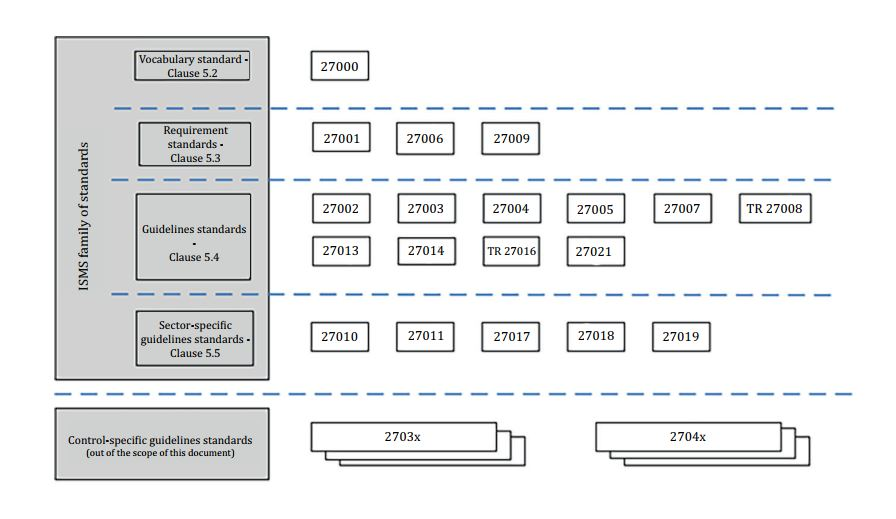
\includegraphics[scale=0.55]{fig/ISO27000.JPG}
    \caption{Família ISO 27000}
    \label{fig:testeISO}
\end{figure}


Conforme ilustrado na Figura~\ref{fig:testeISO}, a família ISO 27000 é organizada entre vocabulário, requisitos, guias e guias específicos.  


\item{Padrão que descreve uma visão geral e terminologia, conforme Figura 2.1:}

\begin{itemize}
    \item ISO/IEC 27000: Mostra uma visão geral da família ISO 27000 além de descrever conceitos básicos como vocabulário, termos e definições.
    \end{itemize}
    
    \item{Padrões que especificam requisitos de segurança, conforme Figura 2.1:}
    
    \begin{itemize}
    \item ISO/IEC 27001: Descreve os requisitos para estabelecer, implementar, operar, monitorar, revisar, manter e melhorar  sistemas de gestão da segurança da informação. 
    \item ISO/IEC 27006 Especifica requisitos para organismos que fornecem auditoria e certificação de sistemas de gestão de segurança da informação. 
    \item ISO/IEC 27009: Define os requisitos para o uso da ISO / IEC 27001 em qualquer setor específico(campo, área de aplicação ou setor de mercado).
    \end{itemize}
    
    \item{Padrões que descrevem diretrizes gerais, conforme Figura 2.1:}
    
    \begin{itemize}
    \item ISO/IEC 27002: Apresenta as melhores práticas que já foram testadas na prática e podem ser adaptadas aos requisitos individuais de cada empresa.
    \item ISO/IEC 27003: Guia de implementação do sistema de gestão de segurança da informação na ISO/IEC 27001.
    \item ISO/IEC 27004: Guia para auxiliar organizações a avaliar a performance da segurança da informação e efetividade do SGSI, para que se esteja de acordo com a  ISO/IEC 27001.
    \item ISO/IEC 27005: Guia para gestão de risco da segurança da informação.
    \item ISO/IEC 27007: Diretrizes para auditoria de sistemas de gestão da segurança da informação.
    \item ISO/IEC TR 27008: Diretrizes para os auditores sobre os controles de segurança da informação. 
    \item ISO/IEC 27013: Guia de orientação sobre a aplicação integrada da ISO / IEC 27001 e ISO / IEC 20000-1. 
    \item ISO/IEC 27014: Guia de princípios e processos para a governança da segurança da informação.
    \item ISO/IEC TR 27016: Gestão de segurança da informação - Economia organizacional
    \item ISO/IEC  27021: Especifica as competências e requisitos necessários para profissionais que atuam com um SGSI.
    \end{itemize}
   \
 \item{Normas que descrevem diretrizes específicas do setor, conforme Figura 2.1:}
 
 \begin{itemize}   
    \item ISO/IEC  27010: Guia da gestão de segurança da informação para as comunicações inter-setoriais e inter-organizacionais
    \item ISO/IEC  27011: Diretrizes de gestão da segurança da informação  para as organizações de telecomunicações com base na norma ISO/IEC 27002. 
    \item ISO/IEC  27017: Diretrizes para controles de segurança da informação aplicáveis ao fornecimento e uso de serviços em nuvem.
    \item ISO/IEC  27018: Código de práticas para proteção de informações de identificação pessoal (PII) em nuvens públicas atuando no processamento de PII.
    \item ISO/IEC T27019: Mostra controles específicos para a indústria de energia.
    
\end{itemize}

Juntos com os demais padrões da família ISO 27000 esses padrões formam um \textit{framework} criado para operar um sistema de gerenciamento da segurança da informação, com base em longas experiências de desenvolvimento \cite{disterer2013}. O foco principal desse TCC é nas ISOs 27001 e 27002 que definem processos para seleção e implantação de controles que ajudam a reduzir os riscos de possíveis vulnerabilidades.


\subsection{ISO 27001}

A norma ISO/IEC 27001 é um padrão internacional que define os requisitos necessários para estabelecer, implementar, manter e melhorar continuamente um SGSI. A norma também inclui requisitos para a avaliação e tratamento de riscos da segurança da informação para a necessidade de cada organização. Os requisitos definidos na norma são genéricos, permitindo que organizações de diferentes tamanhos possam aplicá-los. É importante ressaltar que todos requisitos da seção 4 até o 10 são obrigatórios para que uma organização esteja em conformidade coma a norma. Os controles do "anexo A" {} presentes na ISO/IEC 27001 devem ser implementados se estiverem presentes na declaração de aplicabilidade, juntamente com uma justificativa para inclusão \cite{ISOPDF}. 

A norma ISO/IEC 27001 \cite{ISOPDF} é estruturada da seguinte maneira:

\begin{itemize}
\item Seção 0: Introdução

    Descreve o objetivo da norma e sua importância de integração nos processos da própria organização além de mostrar sua compatibilidade com outras normas de sistemas de gestão.
\item Seção 1: Escopo

    Mostra a abrangência da norma explicando que seus requisitos são genéricos e  que são aplicáveis em qualquer organização, independente do tipo tamanho ou natureza.
\item Seção 2: Referência normativa

    Explica que indispensável a utilização da norma ISO/IEC 27000  como referência para do documento em questão.
\item Seção 3: Termos e definições

    Explica que os termos e definições presentes na ISO/IEC 27000 serão utilizados no documento.
\item Seção 4: Contexto da organização

    A sessão explica que a organização deve determinar questões internas e externas, definir as partes interessadas e seus requisitos, além de definir um escopo da aplicabilidade do SGSI.
\item Seção 5: Liderança

    A sessão explica que a alta direção deve demonstrar sua liderança e comprometimento, estabelecer uma política de segurança de informação  e assegurar que as responsabilidades e autoridades dos papéis relevantes para a segurança da informação sejam atribuídos e comunicados.
\item Seção 6: Planejamento
    Explica que a organização deve determinar riscos e oportunidades que precisam ser consideradas , aplicar um processo de avaliação e tratamento de riscos e definir objetivos da segurança da informação. 
\item Seção 7: Apoio 

    Explica que a organização deve prover recursos necessários para um SGSI, além de determinar competências, conscientizar colaboradores, prover comunicação interna e externa relevantes além de documentar informações.  

\item Seção 8: Operação

    Explica que a organização deve planejar, implementar e controlar processos, para atender os requisitos de um SGSI, além de avaliar e tratar os riscos de segurança da informação.

\item Seção 9: Avaliação do desempenho

    Explica que a organização deve monitorar, medir analisar e avaliar um SGSI, além de realizar auditorias internas. Também é definido uma análise critica pela direção sobre o SGSI para  para assegurar a sua contínua adequação, pertinência e eficácia. 

\item Seção 10: Melhoria
   
    Essa seção explica sobre não conformidades, ação corretiva e melhoria contínua do sistema de gestão
da segurança da informação.

\item Anexo A
   
    Referência aos controles e objetivos de controles presentes na ISO/IEC 27002

 \end{itemize}

%https://advisera.com/27001academy/pt-br/o-que-e-a-iso-27001/

\subsection{ISO 27002}

A norma ISO/IEC 27002 é projetada para ser utilizada como referência na implantação de um SGSI, referente a ISO/IEC 27001 ou como orientação para se implementar controles de segurança baseados em boas práticas. A ISO/IEC 27002 é dividida em 14 seções de controles da segurança da informação, 35 objetivos de controles e 114 controles. A ordem como se encontram as seções não define o grau de importância para cada uma, isso é definido por cada organização que deve identificar a sua aplicabilidade nos processos do negócio \cite{ISO27002}.

%Cada seção de controle da segurança da informação possui um ou mais objetivos de controles. 

A seleção de quais controles da segurança da informação serão usados depende das decisões da organização, baseadas nos critérios para aceitação de risco, nas opções para tratamento do risco e no enfoque geral da gestão de risco presente na organização. Também é importante ressaltar a importância dos controles estarem de acordo com as legislações e regulamentações nacionais e internacionais. A norma em questão é um ponto de partida para o desenvolvimento de diretrizes próprias para a organização. É importante frisar que nem todos os controles e diretrizes presentes na norma podem ser aplicados, pois os mesmos podem não ser relevantes ou suficientes dependendo da análise de risco presente nos requisitos da segurança de informação \cite{ISO27002} .

As seções principais possuem um objetivo de controle, que define o que se espera ser alcançado e um ou mais controles que podem ser usados para se alcançar o seu objetivo de controle. Os controles definem as medidas e ações que devem tomadas para atender ao objetivo de controle, cada controle possui uma diretriz para implementação com informações detalhadas que apoiam a execução do controle. Informações adicionais podem ser mostradas em alguns controles, para apresentar dados de questões legais e referências normativas. As seções, juntamente com seus objetivos, são como segue \cite{ISO27002};

% AQUI SEÇÃO 5
\begin{itemize}
  \item \textbf{Seção 5: Políticas de segurança da informação}
  
    Possui um objetivo de controle: Orientação da direção para segurança da informação.
    
\textit{     \textbf{Orientação da direção para segurança da informação:} }
     
     Tem como objetivo prover orientação da direção e apoio para a segurança da informação de acordo com os requisitos do negócio e com as leis e regulamentações relevantes.
  \end{itemize}
% AQUI SEÇÃO 6
\begin{itemize}
    \item \textbf{Seção 6: Organização da segurança da informação} 
    
    Possui dois objetivos: dispor sobre a  organização interna e sobre os dispositivos móveis e trabalho remoto
    
   \textit{ \textbf{Organização interna:} }
    
    Tem como objetivo estabelecer uma estrutura de gerenciamento, para iniciar e controlar a implementação da segurança da informação dentro da organização.
    
  \textit{  \textbf{Dispositivos móveis e trabalho remoto:}}
    
    Tem como objetivo garantir a segurança das informações no trabalho remoto e no uso de dispositivos móveis.
    
\end{itemize}
% AQUI SEÇÃO 7
\begin{itemize}
    \item \textbf{Seção 7: Segurança em recursos humanos}
    
    Possui três objetivos de controle: Antes da contratação, Durante a contratação e Encerramento e mudança da contratação.
    
  \textit{\textbf{Antes da contratação:}}
    
    Tem como objetivo assegurar que funcionários e partes externas entendem as suas responsabilidades e estão em conformidade com os papéis para os quais eles foram selecionados.

  \textit{\textbf{Durante a contratação:}}
    
    Tem como objetivo assegurar que os funcionários e partes externas estão conscientes e cumprem as suas responsabilidades pela segurança da informação.

    \textit{\textbf{Encerramento e mudança da contratação:} }
    
    Tem como objetivo proteger os interesses da organização como parte do processo de mudança ou encerramento da contratação.
\end{itemize}
% AQUI SEÇÃO 8
\begin{itemize}
    \item \textbf{Seção 8 : Gestão de ativos} 
    
    Possui três objetivos de controle: Responsabilidade pelos ativos, Classificação da informação, Tratamento de mídias.
    
    \textit{\textbf{Responsabilidade pelos ativos:} }
    
    Tem como objetivo identificar os ativos da organização e definir as devidas responsabilidades pela proteção dos ativos.
    
    \textit{\textbf{Classificação da informação:}}
    
    Tem como objetivo assegurar que a informação receba um nível adequado de proteção, de acordo com a sua importância para a organização.
    
    \textit{\textbf{Tratamento de mídias:} }
    
    Tem como objetivo prevenir a divulgação não autorizada, modificação, remoção ou destruição da informação armazenada nas mídias.

\end{itemize}
% AQUI SEÇÃO 9
\begin{itemize}
    \item  \textbf{Seção 9: Controle de acesso}
    
    Possui três objetivos de controle: Requisitos do negócio para controle de acesso, Responsabilidades dos usuários e  Controle de acesso ao sistema e à aplicação.
    
    \textit{\textbf{Requisitos do negócio para controle de acesso:}}
    
    Tem como objetivo limitar o acesso à informação e aos recursos de processamento da informação.
    
  \textit{  \textbf{Gerenciamento de acesso do usuário:}}
    
    Tem como objetivo assegurar acesso de usuário autorizado e prevenir acesso não autorizado a sistemas e serviços.
    
    \textbf{Responsabilidades dos usuários:} 
   
    Tem como objetivo tornar os usuários responsáveis pela proteção das suas informações de autenticação.
    
    \textit{\textbf{Controle de acesso ao sistema e à aplicação:} }
    
    Tem como objetivo prevenir o acesso não autorizado aos sistemas e aplicações.
\end{itemize}
% AQUI SEÇÃO 10
\begin{itemize}
    \item \textbf{Seção 10: Criptografia}
    
    Possui um objetivo de controle: Controle de acesso ao sistema e à aplicação
    
    \textit{\textbf{Controles criptográficos: } }
    
    Tem como objetivo assegurar o uso efetivo e adequado da criptografia para proteger a confidencialidade, autenticidade e/ou a integridade da informação.
\end{itemize}
%------------- AQUI SEÇÃO 11-----------------
\begin{itemize}
    \item \textbf{Seção 11: Segurança física e do ambiente}
    
    Possui dois objetivos de controle: Áreas seguras e Equipamentos.
    
    \textit{\textbf{Áreas seguras:}}
    
    Tem como objetivo prevenir o acesso físico não autorizado, danos e interferências com os recursos de processamento das informações e as informações da organização. 
    
   \textit{ \textbf{Equipamentos:} }
    
    Tem como objetivo impedir perdas, danos, furto ou roubo, ou comprometimento de ativos e interrupção
das operações da organização.
\end{itemize}
% --------------AQUI SEÇÃO 12------------------
\begin{itemize}
    \item \textbf{Seção 12: Segurança nas operações}
    
    Possui sete objetivos de controle: Responsabilidades e procedimentos operacionais, Proteção contra malware, Cópias de segurança, Registros e monitoramento, Controle de software operacional, Gestão de vulnerabilidades técnicas e Considerações quanto à auditoria de sistemas de informação.
    
  \textit{  \textbf{Responsabilidades e procedimentos operacionais:}}
    
    Tem como objetivo Garantir a operação segura e correta dos recursos de processamento da informação.
    
  \textit{  \textbf{Proteção contra malware:}}
    
    Tem como objetivo assegurar que as informações e os recursos de processamento da informação
estão protegidos contra malware.
    
   \textit{ \textbf{Cópias de segurança:}}
    
    Tem como objetivo proteção contra perda de dados.
    
   \textit{ \textbf{Registros e monitoramento:}}
    
    Tem como objetivo registrar eventos e gerar evidências.
    
    \textit{\textbf{Controle de software operacional:}}
    
    Tem como objetivo assegurar a integridade dos sistemas operacionais.
    
    \textit{\textbf{Gestão de vulnerabilidades técnicas:}}
    
    Tem como objetivo prevenir a exploração de vulnerabilidades técnicas.
    
  \textit{  \textbf{Considerações quanto à auditoria de sistemas de informação:}}

     Tem como objetivo Minimizar o impacto das atividades de auditoria nos sistemas operacionais.
\end{itemize}
% --------------AQUI SEÇÃO 13------------------
\begin{itemize}
    \item \textbf{Seção 13: Segurança nas comunicações }
    
    Possui dois objetivos de controle: Gerenciamento da segurança em redes e Transferência de informação.
    
    \textit{ \textbf{Gerenciamento da segurança em redes}}
    
     Tem como objetivo Assegurar a proteção das informações em redes e dos recursos de processamento da informação que os apoiam.

    \textit{ \textbf{Transferência de informação}}
    
     Tem como objetivo Manter a segurança da informação transferida dentro da organização e com
quaisquer entidades externas.
    
\end{itemize}
% --------------AQUI SEÇÃO 14------------------
\begin{itemize}
    \item \textbf{Seção 14: Aquisição, desenvolvimento e manutenção de sistemas}
    
    Possui três objetivos de controle: Requisitos de segurança de sistemas de informação, Segurança em processos de desenvolvimento e de suporte e Dados para teste.
    
    \textit{\textbf{Requisitos de segurança de sistemas de informação}}
    
    Tem como objetivo garantir que a segurança da informação é parte integrante de todo o ciclo de vida dos sistemas de informação. Isto também inclui os requisitos para sistemas de informação que fornecem serviços sobre as redes públicas.
    
   \textit{ \textbf{Segurança em processos de desenvolvimento e de suporte}}
    
    Tem como objetivo garantir que a segurança da informação está projetada e implementada no ciclo de vida de desenvolvimento dos sistemas de informação.
    
  \textit{  \textbf{Dados para teste}}\textit{}
    
    Tem como objetivo assegurar a proteção dos dados usados para teste.
\end{itemize}
% --------------AQUI SEÇÃO 15------------------
\begin{itemize}
    \item \textbf{Seção 15: Relacionamento na cadeia de suprimento}
    
    Possui dois objetivos de controle: Segurança da informação na cadeia de suprimento, Gerenciamento da entrega do serviço do fornecedor.
    
   \textit{ \textbf{Segurança da informação na cadeia de suprimento}}
    
    Tem como objetivo garantir a proteção dos ativos da organização que são acessíveis pelos fornecedores.
    
   \textit{ \textbf{Gerenciamento da entrega do serviço do fornecedor}}
    
    Tem como objetivo Manter um nível acordado de segurança da informação e de entrega de serviços em consonância com os acordos com fornecedores.
\end{itemize}
% --------------AQUI SEÇÃO 16------------------
\begin{itemize}
    \item \textbf{Seção 16: Gestão de incidentes de segurança da informação}
    
    Possui um objetivo de controle: Gestão de incidentes de segurança da informação e melhorias.
    
    \textit{\textbf{Gestão de incidentes de segurança da informação e melhorias}}
    
    Tem como objetivo assegurar um enfoque consistente e efetivo para gerenciar os incidentes de segurança da informação, incluindo a comunicação sobre fragilidades e eventos de segurança da informação.
\end{itemize}
% --------------AQUI SEÇÃO 17------------------
\begin{itemize}
    \item \textbf{Seção 17: Aspectos da segurança da informação na gestão da continuidade do negócio}
    
    Possui dois objetivos de controle: Continuidade da segurança da informação e Redundâncias.
    
    \textit{\textbf{Continuidade da segurança da informação}}
    
    Tem como objetivo a continuidade da segurança da informação deve ser contemplada nos sistemas de gestão da continuidade do negocio da organização.
    
    \textbf{Redundâncias}
    
     Tem como objetivo assegurar a disponibilidade dos recursos de processamento da informação.
\end{itemize}
% --------------AQUI SEÇÃO 18------------------
\begin{itemize}
    \item \textbf{Seção 18: Conformidade}
    
    Possui dois objetivos de controle: Conformidade com requisitos legais e contratuais e Análise crítica da segurança da informação
    
   \textit{ \textbf{Conformidade com requisitos legais e contratuais}}
    
    Tem como objetivo evitar violação de quaisquer obrigações legais, estatutárias, regulamentares ou contratuais relacionadas á segurança da informação e de quaisquer requisitos de segurança.
    
    \textit{\textbf{Análise crítica da segurança da informação}}
    
    Tem como objetivo garantir que a segurança da informação está implementada e operada de acordo com as politicas e procedimentos da organização.
\end{itemize}


\section{Segurança em Ecossistema de Software Móvel}

Bosch e Bosch-Sijtsema \cite{bosch2010integration} definem Ecossistema de Software como uma plataforma de software que consiste em um conjunto de desenvolvedores externos e internos juntamente com uma comunidade que compõem soluções  relevantes para satisfazer suas necessidades.

De acordo com Fontão e colegas \cite{fontao}, Ecossistema de Software móvel é um conjunto de sistemas colaborativos, usuários e desenvolvedores em uma relação de cooperação e competição. Um ECOSs Móvel possui todas as atribuições e conceitos de um ecossistema de software com diferença que ele é voltado para o contexto de dispositivos móveis, nesse caso \textit{smartphones} \cite{mestradoCaio}.

Para Furnell e colegas \cite{furnell2009integrated}, os principais elementos que desafiam a implantação de segurança de informação em organizações são os fatores humanos, organizacionais e tecnológicos. Alguns dos exemplos de fatores humanos são a falta de treinamento ou experiência, cultura da organização. Para fatores organizacionais foram encontrados desafios como estimativa de risco errada, falta de verba, baixa prioridade e distribuição equivocadas das responsabilidades de TI. Finalizando, os desafios tecnológicos são a complexidade do sistema, vulnerabilidades em sistemas e aplicações, falta de eficiência, ferramentas de segurança e mobilidade e distribuição de acesso.

Watanabe \cite{watanabe2017understanding} investigou a vulnerabilidade de aplicativos pagos e gratuitos, descobrindo que 70{\%} dos aplicativos gratuitos e 50{\%} dos aplicativos pagos eram vulneráveis devido a bibliotecas utilizadas no desenvolvimento. Descobriu-se também que aplicativos mais caros/populares tendem a ter mais vulnerabilidades e que aplicativos pagos tendem a não serem atualizados por períodos mais longos do que os aplicativos gratuitos, portanto as bibliotecas vulneráveis nos aplicativos pagos, não são atualizadas por períodos mais longos do que os aplicativos gratuitos.  O ultimo achado identificou que aproximadamente metade das vulnerabilidades detectadas pelas ferramentas de verificação de vulnerabilidade existentes são encontradas em código inacessível.

%rever
Segundo Jaramillo \cite{jaramillo2013cross}, dispositivos \textit{mobile} são criados para serem usados em diversos locais, isso tende a expor o dispositivo a mais riscos de segurança.  Para isso, organizações que usam dispositivos \textit{mobile} em seus serviços devem considerar os seguintes fatores de segurança:
\begin{itemize}
    \item \textbf{Segurança Física:} Quem tem a posse do aparelho, se ele é compartilhado com mais usuários e se o dispositivo já foi roubado ou perdido.
    \item \textbf{Segurança de Acesso:} Que controles garantem que o usuário atual tem acesso a dados e programas do dispositivo.   
    \item \textbf{Segurança de Dados:} Como os dados são protegidos no aparelho. 
    \item \textbf{Segurança de Redes:} Aparelhos \textit{mobile} são expostos a uma grande quantidade redes, que vão desde redes seguras até redes sem segurança alguma. Por essa razão segurança de redes é um ponto muito relevante na criação de um sistema.
    \item \textbf{Uso de Padrões:} Quando o usuário utiliza seu dispositivo tanto para tarefas pessoais ou de trabalho, a organização não consegue controlar ou  pré a provar a instalação de aplicativos que estão ao lado de aplicações disponibilizadas pela organização. 
    \item \textbf{Identidade:} Como assegurar a identidade do usuário e não somente a a do dispositivo rever tradução
\end{itemize}

A grande popularidade faz o sistema operacional Android ser o primeiro alvo de ataques de \textit{malware}. Um dos mecanismos usados pelo sistema para tentar evitar aplicativos maliciosos é o mecanismo de solicitação de permissão, prevenindo acessos em lista de contatos, mensagens de SMS e \textit{e-mails}. Entretanto muitos usuários ignoram os avisos de autorização por considerarem entediante e complicado. Com isso se faz necessário melhorar a efetividade do sistema de permissão, fazendo com que o usuário tenha fácil entendimento dos riscos. \cite{wang2017android}

%Para Fahl \cite{fahl2014hey} a evolução e ascensão das plataformas mobile tem contribuído para o crescimento de lojas de aplicativos (e.g google play, Apple store). Graças a posição de confiança no ecossistema de software, entretanto as mesmas lojas se invadidas representam uma ameaça ao usuário.

%\section{Mapeamento da literatura do uso da família 27000  em ecossistema de software móvel}
